	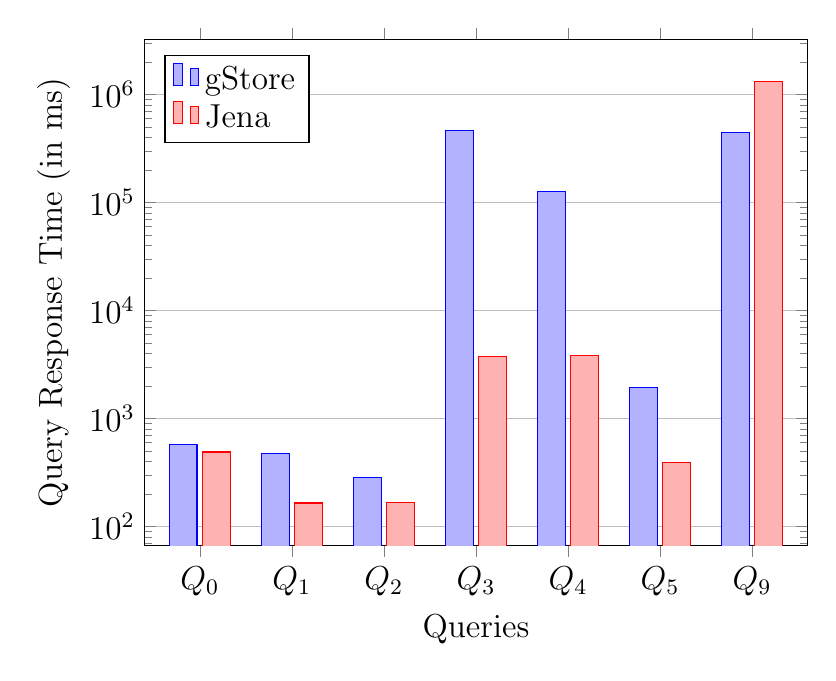
\begin{tikzpicture}[font=\large]
 		 \begin{semilogyaxis}[
               width = 10cm,
               height = 8cm,
    			ybar,
    			%ymin = 1,
    			%ymax = 5000000000,
%    ytick = {1,10,100,1000,10000,100000,1000000,10000000},
   			ymajorgrids = true,
   			ylabel = {Query Response Time (in ms)},
    			xlabel = {Queries},
    			symbolic x coords = {$Q_0$,$Q_1$,$Q_2$,$Q_3$,$Q_4$,$Q_5$,$Q_9$},
    			scaled y ticks = true,
			legend pos= north west,
 legend cell align=left
   		]
   \addplot coordinates {($Q_0$, 578) ($Q_1$, 477) ($Q_2$, 285) ($Q_3$, 465076) ($Q_4$, 127530) ($Q_5$, 1929) ($Q_9$, 447741)};

   \addplot coordinates {($Q_0$, 490) ($Q_1$, 165) ($Q_2$, 166) ($Q_3$, 3727) ($Q_4$, 3847) ($Q_5$, 393) ($Q_9$, 1309775)};

		
   		 \legend{gStore,Jena,Jena}
  		\end{semilogyaxis}
\end{tikzpicture}
